\documentclass[11pt]{article}
%\usepackage[version=3]{mhchem} % Package for chemical equation typesetting
%\usepackage{siunitx} % Provides the \SI{}{} and \si{} command for typesetting SI units
%\usepackage{graphicx} % Required for the inclusion of images
%\usepackage{natbib} % Required to change bibliography style to APA
\usepackage{amsmath} % Required for some math elements 
\usepackage[margin=1in]{geometry}
\usepackage{microtype}
\usepackage[english]{babel}
\usepackage[utf8]{inputenx}
\usepackage{float}
\usepackage{graphics}
\usepackage{graphicx}
\usepackage{subfigure}
\usepackage{amsmath}
\usepackage{textcomp}
\usepackage{makeidx}
\usepackage{hyperref}
\usepackage{braket}
%\usepackage[latin1]{inputenc}
\usepackage{amsthm}
\usepackage{amsfonts}
\usepackage{amssymb}
\usepackage{graphicx}
\usepackage{fullpage}
\usepackage{hyphenat}
\usepackage{float}
\usepackage{longtable}
\usepackage{picture}
\usepackage{multicol}
\usepackage{fancyhdr}
\usepackage{wrapfig}
\usepackage{geometry}
\usepackage{listings}
\usepackage{color}
\definecolor{dkgreen}{rgb}{0,0.6,0}
\definecolor{gray}{rgb}{0.5,0.5,0.5}
\definecolor{mauve}{rgb}{0.58,0,0.82}

\lstset{frame=tb,
	language=C++,
	aboveskip=3mm,
	belowskip=3mm,
	showstringspaces=false,
	columns=flexible,
	basicstyle={\small\ttfamily},
	numbers=none,
	numberstyle=\tiny\color{gray},
	keywordstyle=\color{blue},
	commentstyle=\color{dkgreen},
	stringstyle=\color{mauve},
	breaklines=true,
	breakatwhitespace=true,
	tabsize=3
}

\theoremstyle{theorem}
\newtheorem{theorem}{Theorem}
\newtheorem{proposition}{Proposition}

\theoremstyle{definition}
\newtheorem{definition}{Definition}



%\usepackage{tikz}
%\usetikzlibrary{graphs}
%\usepackage{pgfplots}
%\pgfplotsset{compat=newest}

\setlength\parindent{0pt} % Removes all indentation from paragraphs

\renewcommand{\figurename}{Grafico}
\renewcommand{\tablename}{Tabella}
\newcommand{\at}[2][]{#1\Big|_{#2}}
\renewcommand{\labelenumi}{\alph{enumi}.} % Make numbering in the enumerate environment by letter rather than number (e.g. section 6)

%\usepackage{times} % Uncomment to use the Times New Roman font

%----------------------------------------------------------------------------------------
%	DOCUMENT INFORMATION
%----------------------------------------------------------------------------------------

\title{C1 - Assignment 2 Report: Advection-Diffusion-Reaction equation.} % Title

\author{Student Number: 1894945} % Author name

\date{\today} % Date for the report

\begin{document}

\maketitle % Insert the title, author and date

\begin{center}
C1 - Assignment 2 Report \hfill
Student Number: 1894945
\vspace{3pt} \hrule \vspace{3pt} \hrule
\end{center}

%\clearpage
\tableofcontents

\clearpage
% If you wish to include an abstract, uncomment the lines below
%\begin{abstract}


%\end{abstract}
%\clearpage 

\section{Introduction}

\subsection{Boundary value problem}

\begin{definition}
	\label{defn:BVP}
	Let $\Omega\in\mathbb{R}^{d}$, for $d=\lbrace 1, 2\rbrace$ be a bounded, simply connected, open domain. The Boundary Value Problem (BVP) that will be considered in the following is find, for $f$ and $v$ given, a function $u$ such that 
	\begin{equation}
		\label{eqn:BVP}
		\mathcal{L}[u]=f\hspace{3mm}in\hspace{1mm}\Omega,\hspace{15mm}u=v\hspace{3mm}on\hspace{1mm}\partial\Omega
	\end{equation}
	
	for $\mathcal{L}[u]=-\Delta u(x) + \mathbf{p}(x)\nabla u(x) + q(x)u(x)$, with $\mathbf{p}$ and $q$ given, smooth functions. 
\end{definition}

BVPs like this one are called Dirichlet problems. In what follows, for simplicity, everything will be referred to the case $d=1$. 

\subsection{Finite difference methods}
The discretisations that will be consider in the following are based on the finite difference (FD) approach. The spatial operator $\mathcal{L}$ is evaluated at a set of points $\lbrace x_j\rbrace_{j=1}^{J}$ and the derivatives are replaced with difference quotients of the approximate solution u, which are in turn obtained by truncating (at the desired order of accuracy) the Taylor expansions of the exact solution u(x) around the point $x_j$.\\

Let $\lbrace x_j\rbrace_{j=0}^{J+1}$ be a partition of the interval $(0, L)$, $L\in\mathbb{R}^+$, such that $0=x_0<x_1<\cdots<x_{J+1}=L$. The $j^{th}$ interval will be denoted by $I_j=(x_{j-1}, x_j)$ with mesh size $h_j=|I_j|$. For simplicity, a uniform mesh size will be considered and denoted by $h$, so that $x_j=jh$.\\
Moreover let $u_j$ represents the approximation to the exact solution $u(x_j)$. Then, a simple discrete version of the operator $\Delta$ in \eqref{eqn:BVP} is, for $j=\lbrace 1, \cdots, J\rbrace$, given by:

\begin{align}
	\label{eqn:finite-diff-lap}
	\Delta[u]=\frac{u_{j+1}-2u_j+u_{j-1}}{h^2}
\end{align}

Similarly, the operator $\nabla [u]$ can be discretised as :

\begin{align}
\label{eqn:finite-diff-grad}
\Delta[u]=\frac{u_{j+1}-u_{j-1}}{2h}
\end{align}

Such choices guarantee that the differences between \eqref{eqn:finite-diff-lap} and \eqref{eqn:finite-diff-grad} and their respective continuous counterparts is, at most, $\mathcal{O}(h^2)$, as the following simple calculation explicitly shows. 

\begin{equation}\label{eqn:Taylor-exp}
u(x\pm h)=u(x)\pm hu'(x)+\frac{h^2}{2}u''(x)\pm \frac{h^3}{3!}u'''(x)+\frac{h^4}{4!}u^{(4)}(x)+\mathcal{O}(h^5)
\end{equation}

Inserting Eqn.\eqref{eqn:Taylor-exp} into Eqn.\ref{eqn:finite-diff-lap} and Eqn.\eqref{eqn:finite-diff-grad}, it is easy to see that:

\begin{align}
	\frac{u(x+h)-2u(x)+u(x-h)}{h^2}=u''(x)+\frac{h^2}{12}u^{(4)}(x)+\mathcal{O}(h^4)\\
	\frac{u(x+h)-u(x-h)}{2h}=u'(x)+\frac{h^2}{6}u'''(x)+\mathcal{O}(h^4)
\end{align}

The operators defined in Eqn.\ref{eqn:finite-diff-lap} and Eqn.\eqref{eqn:finite-diff-grad} are \emph{central differences} and will be used for the implementation of the code.\\

The BVP \eqref{eqn:BVP}, can thus be discretised as:

\begin{align}\label{eqn:BVP-discrete}
\begin{split}
-\frac{u_{j+1}-2u_j+u_{j-1}}{h^2}+p_j\frac{u_{j+1}-u_{j-1}}{2h}+q_ju_j=f(x_j), \hspace{5mm}j\in\lbrace 1, \cdots, J\rbrace\\
u_0=v(x_0),\hspace{4mm} u_{J+1}=v(x_{J+1})
\end{split}
\end{align}
	
\subsection{Consistency, convergence and stability of FD methods}
The following discrete function spaces will play an important role in the study of consistency, convergence and stability of FD methods:
\begin{align*}
	&\bar{\mathbb{U}}_h=\lbrace u:\bar{\Omega}_h\rightarrow\mathbb{R}\rbrace\\
	&\bar{\mathbb{U}}^0_h=\lbrace u\in\bar{\mathbb{U}}_h : u|_{\partial\Omega_h}=0\rbrace\\
	&{\mathbb{U}}_h=\lbrace u:\Omega_h\rightarrow\mathbb{R}\rbrace
\end{align*}

where the domain $\bar{\Omega}_h\equiv\lbrace x_j\rbrace_{j=0}^{J+1}$, while $\Omega_h$ represents the set of points in the interior of $\Omega$.\\
It also convenient to introduce the following \emph{restriction operator} $r_h:C(\bar{\Omega})\rightarrow\bar{\mathbb{U}}_h$ defined as:

$$[r_h v]_j=v(x_j),\hspace{5mm}j\in\lbrace 1, \cdots, J\rbrace,\hspace{5mm} v\in C(\Omega)$$

Such an operator allows to compare $C(\bar{\Omega})$ functions with grid functions.\\

Clearly, the discrete problem \eqref{eqn:BVP-discrete} can be now stated as:

\begin{equation}
	\label{eqn:BVP-general-discr}
\end{equation}
$$\bar{\mathcal{L}}_h[u]=f_h$$
where $\mathcal{L}_h:\bar{\mathbb{U}}_h\rightarrow\mathbb{U}_h$ represents both the discretisation of the the different operators involved in Eqn.\eqref{eqn:BVP} and the boundary conditions and $f_h\in\mathbb{U}_h$ is given by $[r_hf]$.\\

\begin{definition}
	\label{defn:consistency}
	The consistency error of the method \eqref{eqn:BVP-general-discr} relative to the exact solution u(x) in a suitable discrete norm is
	$$e_c=||\bar{\mathcal{L}}_h[r_hu]-f_h||_{\mathbb{U}_h} $$
	The discretisation is said to be \emph{consistent} if 
	\begin{equation}
		\label{eqn:consistent}
		e_c\rightarrow 0\hspace{3mm}\text{as}\hspace{3mm}h\rightarrow 0
	\end{equation}
	Moreover, the discretisation is said to be consistent of order $p$ if:
	\begin{equation}
	\label{eqn:consistent-p}
	e_c\rightarrow\mathcal{O}(h^p)\hspace{3mm}\text{as}\hspace{3mm}h\rightarrow 0
	\end{equation}
\end{definition}

\begin{definition}
	The discretisation is said to be \emph{convergent} if 
	\begin{equation}
	\label{eqn:convergent}
	||r_h u-u_h||_{{\bar{\mathbb{U}}}_h}\rightarrow 0\hspace{3mm}\text{as}\hspace{3mm}h\rightarrow 0
	\end{equation}
	The discretisation is said to be \emph{convergent} of order p if 
	\begin{equation}
	\label{eqn:convergent-p}
	||r_h u-u_h||_{{\bar{\mathbb{U}}}_h}\rightarrow \mathcal{O}(h^p)\hspace{3mm}\text{as}\hspace{3mm}h\rightarrow 0
	\end{equation}
\end{definition}

\begin{definition}
	The method is \emph{stable} for some constant $C>0$ if
	\begin{equation}
	\label{eqn:stable}
	||v_h - w_h||_{{\bar{\mathbb{U}}}_h}\le C||\bar{\mathcal{L}}_h[v_h]-\bar{\mathcal{L}}_h[w_h]||_{{{\mathbb{U}}}_h}\hspace{4mm} \forall v_h,w_h\in\bar{\mathbb{U}}_h
	\end{equation}
\end{definition}

The practical meaning of the previous definitions is as follows: Taylor’s theorem gives a way of estimating the consistency error (given a sufficiently smooth exact solution and suitable discretisation of the right hand side), while stability guarantees that rounding errors occurring in the problem will not have an excessive effect on the final result (see \cite{lec-notes}).

\begin{theorem}
	\label{thm:stab-conv}
	Let $u\in\bar{\mathbb{U}}_h$ solve the discrete problem $\mathcal{L}_h[u]=f_h$. If the method is stable and consistent, then it is convergent. 
\end{theorem}
\begin{proof}
	Stability implies:
	$$||r_hu-u||_{{\bar{\mathbb{U}}}_h}\le C ||\bar{\mathcal{L}}_h[r_hu]-\bar{\mathcal{L}}_h[u]||_{{\bar{\mathbb{U}}}_h}=||\bar{\mathcal{L}}_h[r_hu]-f_h||_{{\bar{\mathbb{U}}}_h}$$
	Hence, by consistency, the method is convergent.
\end{proof}

It is worth noticing that the calculation just presented also shows that the order of convergence is at least equal to the order of consistency.\\

\subsection{The present case}
\label{subsec:the-present-case}
In the present assignment, special cases of an 1D linear advection-diffusion-reaction problem are studied. Such equations describe the advection, diffusion and reaction (sometimes the term absorption is used) of a given quantity represented by $u(x)$: typical example can be picked from hydrodynamics and from physics in general.\\
The problem can be formulated as follows. Given $f\in C([0, L])$, find $u\in C^2(0, L)$ such that:

\begin{equation}
	\label{eqn:ass-prob}
	-u''(x)+ pu'(x)+qu(x)= f,\hspace{5mm}u(0)=a, u(L)=b
\end{equation}

for $a, b, p, q\in\mathbb{R}$. \\

Just as the general method previously introduced, the problem can be represented in the matrix form:

\begin{align}
	\label{eqn:matrix-form}
	A\mathbf{u}=\mathbf{f}
\end{align}

where $\mathbf{u}=(u_1, \cdots, u_J)^{T}$, $\mathbf{f}=(f(x_1),\cdots , f(x_J))^{T}$. In this context, the entries of $A$ are given by:

\begin{align}
	\label{eqn:matrix}
	a_{ij} = \begin{cases}
	-\frac{\alpha}{h^2}-\frac{\beta}{2h}, & \text{for } j=i-1\\
	\frac{\alpha}{h^2}+\gamma, & \text{for } j=i\\
	-\frac{\alpha}{h^2}+\frac{\beta}{2h}, & \text{for } j=i+1\\
	0, &\text{otherwise}
	\end{cases}
\end{align}
	
In this way, differential equations can be solved through the methods used in numerical linear algebra.\\

In what follows, it will be assumed that $f=0$,  $p=\frac{\beta}{\alpha}$, $q=\frac{\gamma}{\alpha}$ (for $\alpha, \beta, \gamma\in\mathbb{R}$), $u(0)=0$ and $u(L)=1$.

\subsubsection{The advection-diffusion problem}
\label{subsubsec:ADprob}
If $\gamma$ is set to $0$ in \eqref{eqn:ass-prob}, a simpler problem, composed of only the advection and diffusion terms, is obtained. The solution to such a problem, for $u(0)=0$ and $u(L)=1$ is easily obtained by means of standard techniques for second order ordinary differential equations and reads:

\begin{align}
	\label{eqn:AD-sol}
	u(x)=\frac{1-e^{\frac{\beta}{\alpha}x}}{1-e^{\frac{\beta}{\alpha}L}},\hspace{5mm} 0\le x\le L
\end{align}

It is clear that the solution can be rewritten as a parametric function of the global P\'{e}clet number $\mathbb{P}_e=\frac{|\beta|L}{2\alpha}$, measures the dominance of the advective term over the diffusive one. Setting $L=1$ as required by the assignment instructions and assuming $\beta>0$ for simplicity, one has:

$$	u(x)=\frac{1-e^{2\mathbb{P}_ex}}{1-e^{2\mathbb{P}_e}}, \hspace{5mm} 0\le x\le 1 $$

In order to have a more clear interpretation of the results presented in the following sections, it is worth studying the limit of both large and small global P\'{e}clet number.\\
If $\frac{\beta}{\alpha}<<1$, a simple Taylor expansion up to first order of \eqref{eqn:AD-sol} yields:

\begin{equation}
	\label{key:AD-smallP}
	u(x)\approx\frac{\frac{\beta}{\alpha}x}{\frac{\beta}{\alpha}}=x
\end{equation}

The dominance of $\alpha$ with respect to $\beta$ makes the solution closer to the one of the problem $\alpha u''(x)=0$ with the same boundary conditions (BC). On the other hand, for $\frac{\beta}{\alpha}>>1$ one has:

\begin{equation}
\label{key:AD-bigP}
u(x)\approx\frac{\frac{\beta}{\alpha}x}{\frac{\beta}{\alpha}}=e^{\frac{\beta}{\alpha}(x-1)}=e^{-\frac{\beta}{\alpha}(1-x)}
\end{equation}

Since the exponent is big and negative the solution is almost equal to zero everywhere unless a small neighbourhood of the point $x=1$ where the term $ 1-x $ becomes very small and the solution joins the value $1$ with an exponential behaviour. The width of the neighbourhood is of the order of $\frac{\alpha}{\beta}$ and thus it is quite small: in such an event, we say that the solution exhibits a boundary layer of width $\mathcal{O}\left(\frac{\alpha}{\beta}\right)$ at $x=1$ (see Ref.\cite{numerical-math}).

\subsubsection{The diffusion-reaction problem}
On the other hand, if $\beta$ is set to zero, the solution to the corresponding problem (for the same BC) is given by:

\begin{equation}
	\label{eqn:DR-sol}
	u(x)=\frac{\sinh(\frac{\gamma}{\alpha}x)}{\sinh(\frac{\gamma}{\alpha}L)},\hspace{5mm} 0\le x\le L
\end{equation}

In this case, the relevant parameter to study the dominance of the advection with respect to the response terms, is represented by $D_a=\frac{\gamma}{\alpha}$ and is called Damk\"{o}hler number.\\

\section{The program}
\subsection{Implementation}
The program is built on the class ADR , which stands for Advection-Diffusion-Reaction. The class has 7 private variables: $J$ (the number of points in the interior of $[0,L]$), $\alpha$, $\beta$, $\gamma$ (the parameters associated to the ADR equation at hand), $L$ (the length of the interval), $u_0$ (the boundary condition at $0$) and $u_L$ (boundary condition at $L$). In this way, once the constructor is called, all the variables and parameters defining problem \eqref{eqn:ass-prob} are set.\\
As pointed out in $\S$(\ref{subsec:the-present-case}), BVPs can be solved through numerical methods for linear algebra: the member function \emph{MatrixBuild}, which accepts no argument, constructs matrix $A$ of Eqn.\eqref{eqn:matrix-form}, whose entries are given by \eqref{eqn:matrix}, which will be later inverted through the Gauss-Seidel algorithm. Such a construction takes places within the function \emph{Solver}, that performs the tests required by the assignment instructions through the Gauss-Seidel method and outputs the results on different .txt files. For clarity reasons,  each time a simulation is performed, a suitable success message containing the different parameters of the corresponding test, is printed on the terminal. \emph{Solver} is a member function which accepts 4 arguments and implicitly returns the discretised solution \emph{u$\_$x}. The argument \emph{itCheck} represents the number of iterations after which a check for stagnation of the method is performed, while \emph{MaxIter} represents the maximum number of iterations the user is willing ``wait" and \emph{tol} the given tolerance.\\ 
The member function \emph{An$\_$sol} outputs the analytical solutions at each point of $\Omega_h$, by simply computing either Eqn.\eqref{eqn:AD-sol} or Eqn.\eqref{eqn:DR-sol} at the given set of points. The choice between the two solutions is made by means of an \emph{if} instruction, checking if $\alpha\neq 0, \gamma=0$ or if $\alpha\neq 0, \beta=0$. When none of the above conditions is satisfied, the program exits with an appropriate error message to the user.\\
Discretised and the analytical solutions are finally compared within the function \emph{ADR$\_$Test}. Such a function take as arguments the values of the private datas, the arguments of $Solver$ and the different values of $J$ the user wants to test on. The function loops over them and prints the final error between the numerical solution and the analytical one, in the $L_\infty$ norm, on suitable .txt files, whose names are defined through the parameters the user has set for the test. The ratio between errors obtained for different mesh sizes is computed and printed, too.\\
Since, by means of simply changing the values provided in the main file, both class of equations can be tested with no further modifications to the code, the program can be regarded as particularly flexible.\\

\subsection{Running the program}
The program is run through the Makefile provided. The current optimisation is set to -Ofast and all following tests have been performed with this optimisation choice. Every possible error or warning has been explicitly checked by means of the instruction \emph{-Wall -Wfatal-errors -pedantic} before proceeding to performing the different tests: no warnings appeared.\\
The program generates a fixed number of output files, in which the results of the tests have been stored. Some of these files are used to produce plots by means of six different plotscripts.\\ 

\subsection{Testing correctness}
In order to check the correctness of the implementation of the code, the tests requested by the assignment have been performed. The class of ADR equations chosen as a benchmark is represented by:

\begin{equation}
	\label{eqn:AD}
	-\alpha u''(x)+\beta u'(x) = 0
\end{equation}

Nonetheless, the correctness of the code for the other class of equations is easy to verify by means of changing the parameters in the main file. Such a test, whose results will not be reported here, has been successfully performed in the construction of the code.\\
The solution to Eqn.\eqref{eqn:AD} has been discussed in detail in $\S$(\ref{subsubsec:ADprob}). However, from the numerical point of view, it is important to point out how the presence of a BC implies a suitable modifications of the vector $\mathbf{f}$ to invert against. In fact, if the matrix $A$ is constructed to possess $J$ columns and $J$ rows, since the discrete Laplacian and gradient operators output the value at the point $x_j$ by means of computing functions at the point $x_{j+1}$ and $x_{j-1}$, the values of the function $u(x)$ at the boundary of $\Omega_h$ have to be inserted into the first and last entry of the vector $\mathbf{f}$. Such a construction is performed in the function \emph{Solver} trough the following lines:

\begin{lstlisting}
f[0] = u0_*( ( alpha_/(h*h) ) + ( beta_/(2*h) ) ); //first boundary condition
f[J_-1] = uL_*( ( alpha_/(h*h) ) - ( beta_/(2*h) ) ); //second boundary condition
\end{lstlisting}


Eqn.(\ref{eqn:matrix-form}) then reads:

\begin{align*}
	\begin{pmatrix}
	\frac{\alpha}{h^2}+\gamma & -\frac{\alpha}{h^2}-\frac{\beta}{2h} & 0 & 0 & 0 & \cdots & 0 & 0\\
	-\frac{\alpha}{h^2}+\frac{\beta}{2h} & \frac{\alpha}{h^2}+\gamma & -\frac{\alpha}{h^2}-\frac{\beta}{2h} & 0 & 0 & \cdots & 0 & 0\\
	0 & -\frac{\alpha}{h^2}+\frac{\beta}{2h} & \frac{\alpha}{h^2}+\gamma & -\frac{\alpha}{h^2}-\frac{\beta}{2h} & 0 & \cdots & 0 & 0\\
	\vdots & \vdots & \ddots & \ddots & \ddots & \cdots & \vdots & \vdots \\
	0 & 0 & \cdots & \cdots & \cdots & \cdots &  \frac{\alpha}{h^2}+\gamma & -\frac{\alpha}{h^2}-\frac{\beta}{2h}\\
	\end{pmatrix}
	\begin{pmatrix}
	u_1\\
	\vdots\\
	\\
	\vdots\\
	u_{J-1}\\		
	\end{pmatrix}
	=
	\begin{pmatrix}
	u_0\left(-\frac{\alpha}{h^2}+\frac{\beta}{2h}\right)\\
	0\\
	\vdots\\
	0\\
	u_{L}\left(-\frac{\alpha}{h^2}-\frac{\beta}{2h}\right)\\		
	\end{pmatrix}
\end{align*}

where $\mathbf{u}$ is the initial guess required by the Gauss-Seidel algorithm to work. In the present case, each component of $\mathbf{u}$ has been set to $0$, so that $u_j=0\hspace{3mm}\forall j\in\lbrace 1,\cdots, J\rbrace$.\\
Solutions to  Eqn.\eqref{eqn:AD} have been obtained for different values of the mesh size $h=\frac{1}{J+1}$ and different values of the $\mathbb{P}_e$. The error, i.e the distance between the exact solution on the grid and the approximate one in the $L_\infty$ norm, is computed for each solution. As previously mentioned, the ratio between such errors for two successive solutions of the same problem (same $\mathbb{P}_e$, but different $h$) have been computed: the reason for this will be clear in the next sections.\\




\subsection{Results of the tests}
In the following, the results of the more significant tests performed will be reported and briefly discussed. The tolerance has been set to $10^{-6}$ for each of the tests, while the values of \emph{itCheck} and \emph{MaxIter} are kept fixed to $10^4$ and $10^9$ respectively.\\

\subsubsection{Solutions to the AD equation}
The \emph{ADR$\_$test} function has been shown to work correctly for the following  P\'{e}clet numbers:
$$\mathbb{P}_e=\lbrace 0.0000, 0.0005, 0.0100, 1.0000, 10.5000 \rbrace$$
The solutions $u(x)$ obtained for the different cases, indexed by the value of $J$ chosen, can be found in the files $P\_numb\_...\_Solution\_J\_....txt$ , where the dots stand for the different possible values of $\mathbb{P}_e$ and $J$. The residual error at every iteration, in the $L_\infty$ norm, is stored in the files $P\_numb\_...\_Residual\_J\_....txt$, which provide a direct proof of the general correctness of the code.\\
Finally, the distance between the exact solution and the approximate one, in the $L_\infty$ is printed on \emph{Errors$\_$P$\_$numb$\_$...txt} files. Unsurprisingly, the error becomes smaller as the mesh size decreases.\\
The correctness of the algorithm has been tested for different values of $h$, as required by the assignment. The values of the mesh size have been chosen to be:

$$h=\lbrace10, 20, 40, 80, 160, 320, 640\rbrace$$

Keeping the P\'{e}clet number fixed, the same equation has been solved for all the previous mesh sizes. The results are reported in the following.\\


\subsubsection{Small P\'{e}clet numbers}
Solutions to to Eqn.\eqref{eqn:AD} have been studied in the case of small $\mathbb{P}_e$, as required by the assignment. The obtained results are reported in the following plots.
\begin{figure}[H]
	\begin{center}
		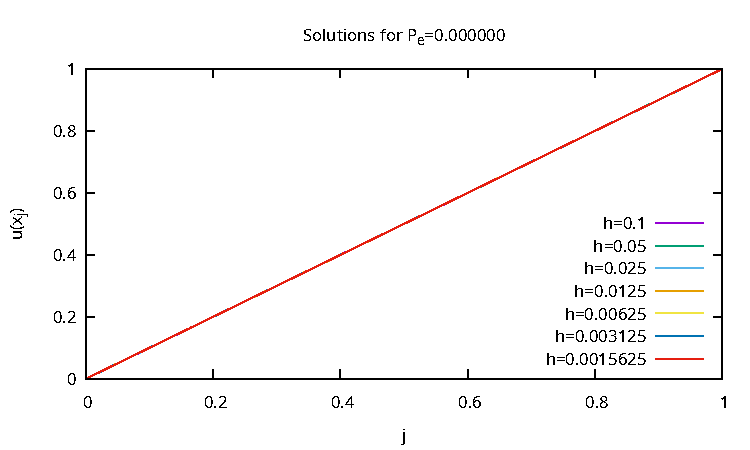
\includegraphics[width=0.87\textwidth]{ADRsol5.pdf}
	\end{center}
	\caption{Graphical representation of the solution to Eqn.\eqref{eqn:AD} for $\alpha=1.0$ , $\beta=0.0$. The solutions for different mesh sizes overlap, so that only the last one is distinguishable.
		\label{fig:P_0}}
\end{figure}

\begin{figure}[H]
	\begin{center}
		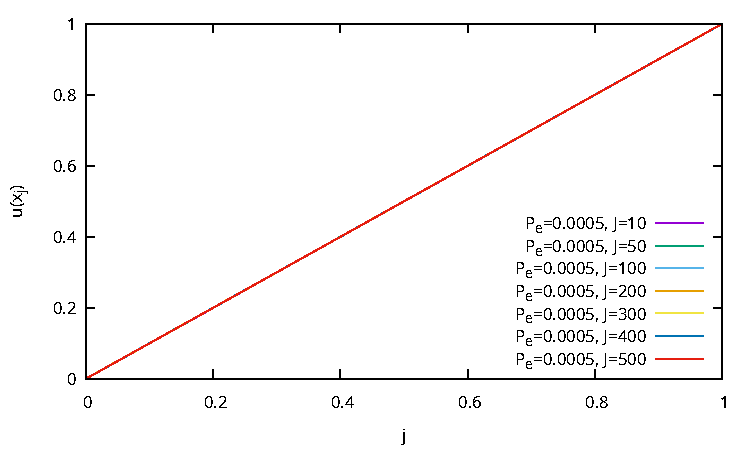
\includegraphics[width=0.87\textwidth]{ADRsol1.pdf}
	\end{center}
	\caption{Graphical representation of the solution to Eqn.\eqref{eqn:AD} for $\alpha=1000$ , $\beta=1$. The solutions for different mesh sizes overlap, so that only the last one is distinguishable.
		\label{fig:P_0.0005}}
\end{figure} 

\begin{figure}[H]
	\begin{center}
		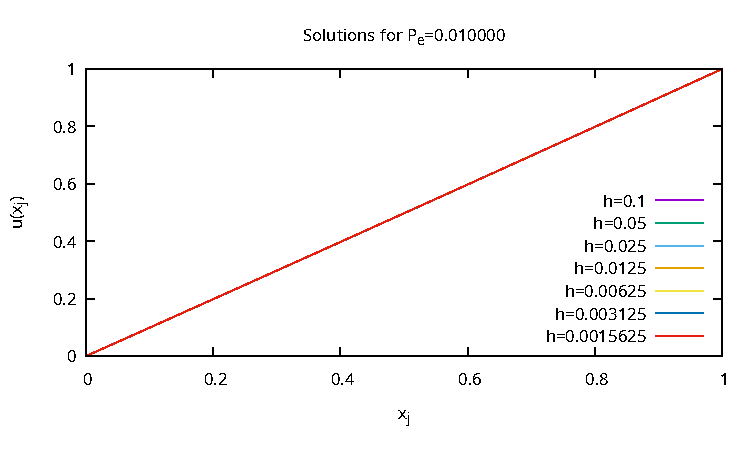
\includegraphics[width=0.9\textwidth]{ADRsol4.pdf}
	\end{center}
	\caption{Graphical representation of the solution to Eqn.\eqref{eqn:AD} for $\alpha=10.0$ , $\beta=0.1$. The solutions for different mesh sizes overlap, so that only the last one is distinguishable.
		\label{fig:P_0.01}}
\end{figure} 

The solutions appear to be straight line on the interval $[0, 1]$. Remembering what has been discussed in $\S$(\ref{subsubsec:ADprob}), such a result does not appear surprising: Fig.\ref{fig:P_0.0005} and Fig.\ref{fig:P_0.01} show the rightfulness of the Taylor expansion performed in Eqn.\eqref{key:AD-smallP}. Finally, Fig.\ref{fig:P_0} shows that the code is able to find the correct solution to the problem also in the case of $\beta=0$. In fact, under these circumstances, Eqn.\eqref{eqn:AD} simplifies to:

$$-\alpha u''(x)=0$$

which, for the given BCs, admits the unique solution $u(x)=x$.\\

\subsubsection{P\'{e}clet number close or equal to 1}
Solutions to Eqn.\eqref{eqn:AD} have been studied in the case $\alpha=0.25, \beta=0.5$ as well. Such a choice of the parameters results in $\mathbb{P}_e=1$. The result is reported in the following plot.

\begin{figure}[H]
	\begin{center}
		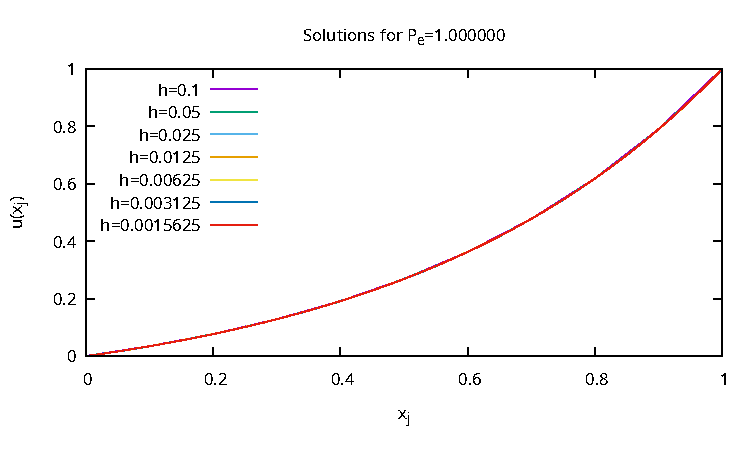
\includegraphics[width=0.9\textwidth]{ADRsol2.pdf}
	\end{center}
	\caption{Graphical representation of the solution to Eqn.\eqref{eqn:AD} for $\alpha=0.25$ , $\beta=0.5$.
		\label{fig:P_1}}
\end{figure}

The exponential behaviour of the solution is now evident. In fact, in the present case, the Taylor expansion of the exponential function around 0 cannot be truncated after the first term being that $\frac{\beta}{\alpha}=1$.\\
Solutions overlap in this case as well, but small differences between them are noticeable for big enough j: by means of a suitable zoom on the plot, it is possible to see that the red and blue curve present a slightly different profile.\\

\subsubsection{Large P\'{e}clet number}
Finally, solutions to Eqn.\eqref{eqn:AD} have been studied in the case of large $\mathbb{P}_e$. The result is reported in the following plot.

\begin{figure}[H]
	\begin{center}
		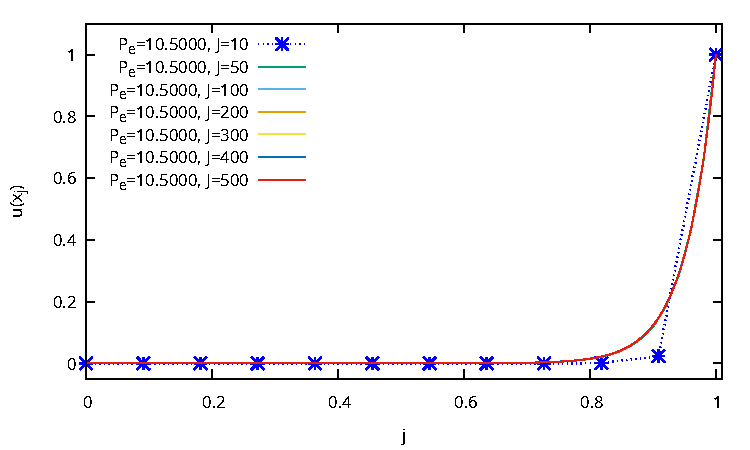
\includegraphics[width=1.0\textwidth]{ADRsol3.pdf}
	\end{center}
	\caption{Graphical representation of the solution to Eqn.\eqref{eqn:AD} for $\alpha=1.0$ , $\beta=21.0$. The solutions overlap for $h\ge 0.025$.
		\label{fig:P_10.5}}
\end{figure}

The choice of the values of $\alpha$and $\beta$ has been made through the following criterion.\\
A sufficient condition for the Gauss-Seidel method to converge is that the matrix $A$ which the algorithm has to invert is strictly diagonally dominant (see \cite{numerical-math}). In the present case, such a condition is satisfied if:

$$\left\|\frac{2\alpha}{h^2}\right\|> \left\|\frac{\alpha}{h^2}+\frac{\beta}{2h}\right\| + \left\|-\frac{2\alpha}{h^2}+\frac{\beta}{2h}\right\|$$

However:

$$\left\|\frac{\beta}{h}\right\|= \left\|-\frac{\alpha}{h^2}+\frac{\beta}{2h}+\frac{\alpha}{h^2}+\frac{\beta}{2h}\right\|\le $$

So that, in order to have strict diagonally dominance, it must be:

$$\left\|\frac{\beta}{h}\right\|<\left\|\frac{2\alpha}{h^2}\right\|$$

Hence, for $L=1$, remembering that $h=\frac{1}{J+1}$, one has that a sufficient condition for the Gauss-Seidel method to converge is:

$$J>\mathbb{P}_e-1$$

The choice of $\alpha=1$ and $\beta=21$ satisfy the above condition. It was explicitly checked during the construction of the program that the choice of a great $\beta$ greater (e.g. $\beta=1000$) does not allow the algorithm to converge and the program exits with an appropriate warning to the user. Clearly, large values of $\beta$ can be tested with large enough $J$, so that the previous inequality is satisfied.\\

\subsection{Error analysis and order of convergence}
As required by the assignment, errors on the solution have been computed and analysed. Not surprisingly, the distance between analytical and the approximate solution becomes smaller when the mesh size decreases.\\
The study of such errors becomes of great importance to determine the order of convergence of the method. Assume the FD method here used is consistent of order p, then:

$$\left\|\frac{\mathcal{L}_h[r_hu]-f_h}{\mathcal{L}_{\frac{h}{2}}\left[r_\frac{h}{2}u\right]-f_\frac{h}{2}}\right\|=\frac{Ch^p+\mathcal{O}(h^{p+1})}{C\left(\frac{h}{2}\right)^p+\mathcal{O}(h)^{p+1}}=2^p$$

where $\mathcal{O}(h^{p+1})$ terms were neglected.\\
\section{Conclusive remarks}
In this section some additional comments and observation are presented.

\subsection{Memory}
When dynamically allocating memory, one has always to make sure to free the reserved locations as soon as they are no longer needed. With the help of the software \emph{valgrind}, possible memory leaks have been checked. To do this, is it necessary to compile with \emph{-g} and \emph{-O1} optimisation. After having compiled the program, the following instruction has been used:

\begin{verbatim}
$ valgrind --leak-check=yes ./sparsematrix
\end{verbatim}

The following output has been produced on the terminal:

\begin{verbatim}
==4200== Memcheck, a memory error detector
==4200== Copyright (C) 2002-2017, and GNU GPL'd, by Julian Seward et al.
==4200== Using Valgrind-3.13.0 and LibVEX; rerun with -h for copyright info
==4200== Command: ./sparsematrix
==4200== 
==4200== 
==4200== HEAP SUMMARY:
==4200==     in use at exit: 0 bytes in 0 blocks
==4200==   total heap usage: 1,252,428 allocs, 1,252,428 frees, 989,616,540 bytes allocated
==4200== 
==4200== All heap blocks were freed -- no leaks are possible
==4200== 
==4200== For counts of detected and suppressed errors, rerun with: -v
==4200== ERROR SUMMARY: 0 errors from 0 contexts (suppressed: 0 from 0)
\end{verbatim}

One can clearly see that no memory has been lost, so that everything has been deleted correctly. \\
It may seem a little strange at fist that all the heap blocks were freed, even though no explicit call to the destructor has been made. However, all instances are built by the function Gauss$\_$Seidel$\_$test, so that the deletion is automatically performed every time the programs exits the function.\\
The absence of memory leaks is however non trivial, since it proves that the destructor has been constructed correctly. This can be explicitly checked by means of commenting out the last two lines of the destructor: if \emph{valgrind} is called again, some memory leak will be found.\\ 


\subsection{Performances}
\label{subsec:perf}
In order to test performance, the following instructions have been used\footnote{The test has been performed only on the part of the code concerned with the test over different $\lambda$ and $\delta$, commenting out the part on different $N$ in the main file. }:
\begin{verbatim}
$ valgrind --tool=callgrind ./sparsematrix
$ kcachegrind
\end{verbatim}

The first command analyses the perfomances in the terms of load distrubution, while \emph{kcachegrind} is used to visualise the load distribution results. Results are reported in the following screenshot.


It is clear that a better efficiency could have been obtained if the program had not relied so much on the \emph{getValue} function, which is not particularly efficient.\\

\subsubsection{Possible solutions}
A possible way to optimise the code is to sort the indexes and values as soon as they are entered, so that each index can be associated to the corresponding value in a unique way and without the necessity to call a the \emph{getValue}. Such a solution, however, has not been implemented, since even though it is clearly more efficient for the matrix given in the assignment, it is not immediately clear how faster and optimised the code could become in the case of denser sparse matrix. On the other hand, it is still reasonable to expect that such a choice will make the program faster, since the sorting takes place only at the beginning of the program and \emph{getValue} is called a large number of times during the iterations.\\
Possibly, the best solution is to store the values and the indexes by means of the \emph{insert} function instead that through a \emph{push$\_$back}: this way, the values
 will be automatically sorted.\\



\cleardoublepage
%\add1contentsline{toc}{chapter}{\bibname}
\begin{thebibliography}{99}

\bibitem{numerical-math} A. Quateroni, R. Sacco, F. Saleri;
\emph{Numerical Mathematics}, Vol.37, Springer Verlag, (2007).

\bibitem{lec-notes} T. Grafke;
\emph{Scientific Computing}, Lecture Notes, University of Warwick, (2018).







\printindex
\end{thebibliography}
\bibliography{bibliography} % BibTeX database without .bib extension
\end{document}



%----------------------------------------------------------------------------------------
%	BIBLIOGRAPHY
%----------------------------------------------------------------------------------------

%\bibliographystyle{apalike}

%\bibliography{sample}

----------------------------------------------------------------------------------------


%end{document}